
\documentclass{article}

% Recommended, but optional, packages for figures and better typesetting:
\usepackage{microtype}
\usepackage{graphicx}
\usepackage{subfigure}
\usepackage{booktabs} % for professional tables
\usepackage{makecell}
\usepackage{amssymb}

% hyperref makes hyperlinks in the resulting PDF.
% If your build breaks (sometimes temporarily if a hyperlink spans a page)
% please comment out the following usepackage line and replace
% \usepackage{icml2019} with \usepackage[nohyperref]{icml2019} above.
\usepackage{hyperref}

% Attempt to make hyperref and algorithmic work together better:
\newcommand{\theHalgorithm}{\arabic{algorithm}}

% Use the following line for the initial blind version submitted for review:
% \usepackage{icml2019}

% If accepted, instead use the following line for the camera-ready submission:
\usepackage[accepted]{icml2019}

% The \icmltitle you define below is probably too long as a header.
% Therefore, a short form for the running title is supplied here:
\icmltitlerunning{On the Robustness of Training with Frozen Layers}

\begin{document}

\twocolumn[
\icmltitle{The Cold Never Bothered Me Anyway: \\On the Robustness of Training with Frozen Layers}

\icmlsetsymbol{equal}{*}

\begin{icmlauthorlist}
\icmlauthor{Dori Medini}{}
\icmlauthor{Gal Shachaf}{}
\icmlauthor{Noam Loya}{}
\end{icmlauthorlist}

\vskip 0.3in
]

\begin{abstract}
Do we need an abstract?
\end{abstract}
\section{Introduction}
 - Present the question of generalization vs. over parameterization\\
 - Recent works on the role of initialization in generalization\\
 - Singer - split layers into critical and robust\\
 - Experiments with freezing\\
 - Combining all together: What we are doing.\\
 \cite{learningNothing} has a good introduction, use that\\
We attempt to further investigate the robustness affect.\\
 The rest of the paper is organized as follows:\\
First, related work is presented on section \ref{relatedWork}. Then, on section \ref{setting}, we describe our experiment framework and introduces terminology used throughout the paper. Sections \ref{training} and \ref{freezingRobustness} examine the effect of training with frozen layers on training and on robustness, divided to models and datasets. On section \ref{regularization} we study the effects of regularization methods on robustness. On section \ref{winnerySection} we discuss the relation of robustness to the lottery ticket hypothesis. On section \ref{transfer} we attempt to apply robustness for transfer learning. Finally, section \ref{conclusion} concludes this paper and discuss future direction.  


\section{Related Work}\label{relatedWork}
Tackling the question of generalizing well while having a large number of parameters, \cite{intrinsic} found that using a small number of parameters (the \textit{intrinsic dimension}) projected into a larger space using a random matrix can lead to good generalization. \cite{sgdAlign} have studied properties of Gradient Descent algorithm that contribute to generalization.\\
Recent works have also demonstrated that a well-initiated subset of a network can yield good performance: \cite{frankle2018lottery} used pruning techniques to uncover a \textit{"winning ticket"}: a subset of weights whose initialization allow them to train effectively, and even achieve better performance when trained separately. \cite{lotteryAtScale} have shown that the winning ticket is more stable if the pruning is done at an early stage of training instead on the initial weights. Building upon them, \cite{generalizingLottery} have successfully used the same winning ticket for multiple image datasets, and using different optimizers.\\
As mentioned, \cite{allLayers} have studied the role of different layers. By re-initialization and measuring the change in performance, they identified \textit{critical} and \textit{ambient} layers (\textit{robust} in early versions). Critical layers are very sensitive to re-initialization, while resetting ambient layers is negligible.\\
Others have studied "freezing" weights: fixing a subset of the weights, and training the rest of the network normally. \cite{freezeout} used layer freezing in order to accelerate training. \cite{fixLastLayerToHadamard} have shown that using a fixed Hadamard matrix as the last layer do not decrease performance. Later, \cite{learningNothing} fixed the majority of network parameters, while still preserving high accuracy. 

\section{Setting} \label{setting}
We follow the same framework as \cite{allLayers}, to analyze the behaviour of different layers. We trained various types of neural networks with stochastic gradient descent for 100 epochs. All network weights are initialized randomly (TODO: distribution?). After a model is trained, we measure robustness of individual layers by the following two procedures:\\
\emph{Re-initialization:} Setting a layer's weights to a given epoch's weights, and not modifying the other layer's weights. We measure robustness to re-initialization by the change in test accuracy before and after re-initialization, without any further training or tuning of network parameters. A layer that is highly sensitive to re-initialization is said to be \emph{critical}, and a layer that is not very sensitive to this procedure is called \emph{ambient}. While these aren't well-defined terms, there is no ambiguity in classifying layers in the empirical results. \\
\emph{Re-randomization:} Re-sampling random values to a layer's weights, from the same initial distribution. \\
\begin{figure}
  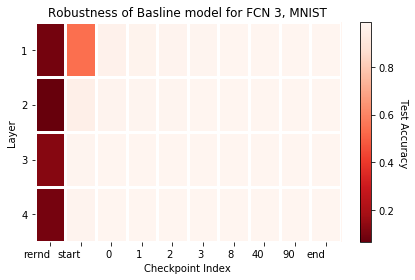
\includegraphics[width=\linewidth]{images/baseline_fc3_mnist_heatmap.png}
  \caption{Baseline robustness results for 3-layered FCN. Test performance when setting a layer weights (rows) to the checkpoint index weight (columns) the first column shows robustness w.r.t re-randomization.}
  \label{fig:baseline_fc3_heatmap}
\end{figure}
Figure \ref{fig:baseline_fc3_heatmap} demonstrates robustness measurements on a baseline model, 3 layered fully connected network (FCN 3) on MNIST. As in \cite{allLayers}, we can see that the bottom (first) layer is critical and is most sensitive to  re-initialization. The rest of layers are ambient, and are not as sensitive. Re-randomization of all layers decreases performance (test accuracy) severely.\\
Our experiments involve \emph{layer freezing}: fixing layer weights throughout training. TODO: elaborate. what happens to gradients?\\
All our experiments were performed in Tensorflow \cite{tensorflow2015-whitepaper}, TODO: any other information? CPU-GPU, types..\\
TODO: type of networks trained, datasets, optimizers, loss....

\section{The effect of freezing layers on training} \label{training}
\subsection{Fully Connected Network on MNIST}
We start by examining performance when training the network while freezing layers. Clearly, freezing layers during training effects the accuracy \cite{freezeout}. But it is interesting to note that the decrease in performance differs between critical and ambient layers, and can be observed in table \ref{tab:test_accuracies_by_frozen} and figure \ref{fig:fc3_training}.\\
When an ambient layer is frozen, results are almost equal to the baseline results. On the other hand, when a critical layer is frozen we have a larger decrease in performance, a drop which is equivalent to when \emph{all} ambient layers are frozen. The significant drop when the critical layer is frozen might be due to the loss of information caused by freezing the first layer. \\
Observing training speed reveals interesting phenomena as well: while freezing ambient layers has no effect on training speed, freezing the critical layer has a major effect. This is somewhat counter-intuitive, as the bottom layer takes longest to train (TODO reference). When all the ambient layers are frozen, training takes longest, which is probably due to the fact that only the bottom layer is trained. (TODO elaborate)\\
This effect appears on a 5-layer fully connected network as well.\\
\begin{table}[h!]
  \begin{center}
    \label{tab:test_accuracies_by_frozen}
    \begin{tabular}{l|c|c|r} % <-- Alignments: 1st column left, 2nd middle and 3rd right, with vertical lines in between
      \makecell{\textbf{Frozen}\\ \textbf{Layers}} & \makecell{\textbf{Test}\\ \textbf{Accuracy}} & \makecell{\textbf{Distance}\\ \textbf{from} \\ \textbf{baseline}} & \makecell{\textbf{Epochs}\\ \textbf{to 97.5\%}}\\
      \hline
      \makecell{No frozen layers} & \makecell{0.9856} & \makecell{0.0} & \makecell{2}\\ 
      \makecell{Critical layer (1)} & \makecell{0.9751} & \makecell{0.0105}& \makecell{17}\\
      \makecell{Single ambient layer\\ 
      (2,3,4 average) }
        & \makecell{0.9829} & \makecell{0.002}& \makecell{2}\\
      \makecell{All ambient layers\\ (2,3,4)} &  \makecell{0.9774} & \makecell{0.0082} & \makecell{53}
      
    \end{tabular}
\caption{Test accuracy on 3 layered fully connected network on MNIST, by frozen layers during training.} 
  \end{center}
\end{table}

\begin{figure}
  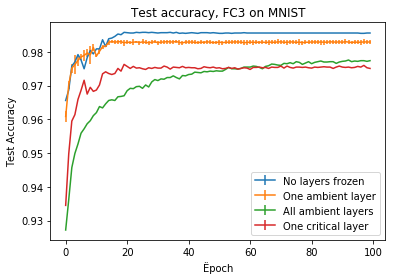
\includegraphics[width=\linewidth]{images/fc3_mnist_training_plots.png}
  \caption{Test accuracy by epoch, for different sets of layers frozen during setting. The critical layer is the first layer, and the rest of the layers are ambient (based on \ref{fig:baseline_fc3_heatmap}). The ambient layers are averaged and the error bars are the standard deviation.}
  \label{fig:fc3_training}
\end{figure}
\subsection{Fully Connected Newtork on CIFAR 10}
% Robustness pattern is a little different when training on CIFAR, probably since it is a more complex dataset (TODO: rephrase and reference).  
\subsection{Small Convolutional Network on CIFAR 10}
% Figure \ref{fig:cnn_cifar_training_patterns} presents the robustness pattern hen training a small CNN on CIFAR 10.\\
% The effects of freezing layers is quite similar to the effects that occurred on MNIST. 
\section{Robustness with frozen layers} \label{freezingRobustness}
\subsection{Fully Connected Network on MNIST}
We examine the robustness effect when training with frozen layers. We trained a fully connected network, while freezing a layer (or a set of layers) throughout training. Then we apply re-initialization and re-randomization to measure robustness. We compare all the results to the robustness of a baseline model trained without freezing any layers.\\
When training a baseline fully connected network with 3 layers on MNIST (figure \ref{fig:baseline_fc3_heatmap}), it is notable the first layer is critical while the other layers are ambient, and all layers are sensitive to re-randomization as in \cite{allLayers}.\\
Another interesting phenomenon is that freezing layers during training changes the effect in different ways corresponding to the frozen layer's robustness (figure \ref{fig:fc3_drop_by_layer_type}):\\ 
\begin{figure}
  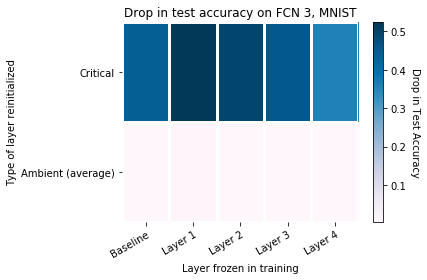
\includegraphics[width=\linewidth]{images/fc3_mnist_drop_in_acc_by_layer.png}
  \caption{Robustness by frozen layers and reinitialized layer type. Drop in test accuracy for each model trained with a different frozen layer (columns), when the corresponding type of layer (rows) is re-initialized to epoch 0. For ambient layers, the average is presented, with STD $<$ 0.001 for all set of layers. (TODO: validate!)}
  \label{fig:fc3_drop_by_layer_type}
\end{figure}
\emph{Freezing a critical layer:} When freezing the first layer, the proceeding layer "substitutes" for it and becomes more critical than the first layer was before freezing. Re-initializing the first layer on the baseline model drops test accuracy from 98.5\% to 54\%. On the first layer frozen model, re-initializing the second layer demonstrates a larger decrease in test accuracy: from 97.5\% to 45\%. Not only the effect is stronger, but it lasts for more epochs too: on the baseline model, the effect almost vanishes when resetting the first layer to the second epoch weights (98.5\% drops to 97.7\%). When the first layer is frozen, resetting the second layer weights to the second epoch checkpoint shows a larger drop in performance (97.5\% drops to 95.5\%).\\
\emph{Freezing an ambient layer:} When  an ambient layer is frozen during training, we have a small "smoothing" effect: the previously ambient layers become more critical and the previously critical layer is a little less critical. For instance, when layer 3 is frozen during training re-initialization of the critical layer drops test accuracy from 98.2\% to 52.2\% , as opposed to the baseline model, where the drop is slightly smaller: from 98.5\% to 54.3\%. Re-initializing an ambient layer drops test accuracy from 98.2\% to 91.3\% on average, a larger decrease than the baseline model (98.5\% to 96.5\% on average). This effect is consistent for all ambient and becomes stronger as the frozen layer is closer to the output layer.\\    TODO: add average ambient layers statistics\\
We also trained while freezing the first and second layers, thus not allowing the second layer to substitute for the first, critical layer. In this case, the third layer becomes critical, and the effect lasts for even more epochs: resetting the layer weights to later epochs also harms model's performance (figure \ref{fig:f12_fc3_heatmap}).\\
The same effect occurs when training a 5-layer fully connected network on MNIST. \\
\begin{figure}
  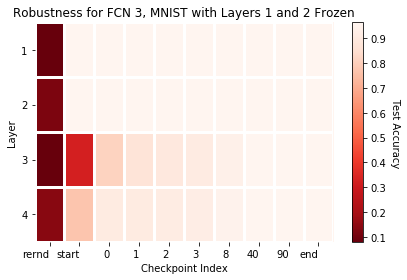
\includegraphics[width=\linewidth]{images/f12_fc3_mnist_heatmap.png}
  \caption{Robustness results for 3-layered FCN trained with layer 1 and 2 frozen.}
  \label{fig:f12_fc3_heatmap}
\end{figure}
% \begin{figure}
%   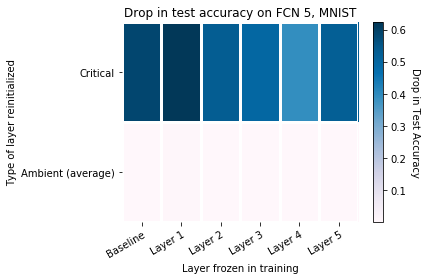
\includegraphics[width=\linewidth]{images/fc5_mnist_drop_in_acc_by_layer.png}
%   \caption{Robustness by frozen layers and reinitialized layer type, on a 5 layer FCN with MNIST. Drop in test accuracy for each model trained with a different frozen layer (columns), when the corresponding type of layer (rows) is re-initialized to epoch 0. For ambient layers, the average is presented, with STD $<$ 0.001 for all set of layers. (TODO: validate!)}
%   \label{fig:fc5_drop_by_layer_type}
% \end{figure}
\subsection{Fully Connected Network on CIFAR 10}
\section{Robustness with regularization} \label{regularization}
Different methods of regularization seem to have different effect on robustness. We experimented with l1 regularization, l2 and Dropout \cite{dropout}, both with and without freezing layers.\\
L2 regularization seems to have a smoothing effect (figure \ref{fig:fc3_l2_drop_by_layer_type}). All layers become more critical, while still preserving the order: the critical layer on the baseline remains the most critical with regularization, and layers become more ambient as we move further from the critical layer. When we add layer freezing to training, the effect changes depending on the frozen layer. When the first, most critical layer is frozen, we have a similar effect: all layers become more critical, where the second layer is most critical and the output layer is most ambient. TODO: repeat this experiment and see if results are consistent. Explain the other layers.\\


\begin{figure}
  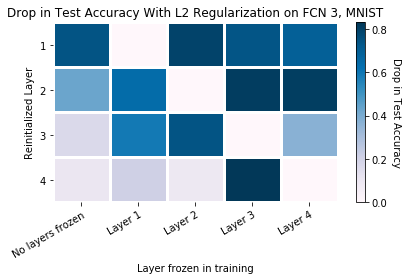
\includegraphics[width=\linewidth]{images/fc3_mnist_l2_reg_drop_in_acc_by_layer.png}
  \caption{Robustness by frozen layers and reinitialized layer, on a 3 layer FCN with MNIST, trained with L2 regularization. Drop in test accuracy for each model trained with a different frozen layer (columns), when the corresponding type of layer (rows) is re-initialized to epoch 0.}
  \label{fig:fc3_l2_drop_by_layer_type}
\end{figure}        

\section{Robustness and the lottery ticket hypothesis} \label{winnerySection}
    
In \cite{frankle2018lottery}, using pruning techniques they isolated a well initialized sub-network that trains faster and even achieves better results on data, a \emph{winning ticket}. \cite{allLayers}, on the other hand, show that layers differ in their sensitivity to initialization. We wanted to investigate the relationship between the two: is a weight in a critical or an ambient layer is more likely to be a part of a winning ticket? Also, since a winning ticket has better initialization, does it have different robustness pattern? \\
As in \cite{frankle2018lottery}, we used pruning to reveal the winning ticket from a trained model, removing any weight that's larger than a certain threshold. The threshold constant itself was chosen s.t. a non-negligible portion of weights were pruned and the accuracy changed by $\lessapprox 1\%$; and as the weights were drawn using Glorot initialization the threshold was multiplied by $\sqrt{\frac{2}{fanin + fanout}}$ when pruning a specific layer. After pruning, we re-initialized the remaining weights, trained the pruned model and successfully replicated the results of \cite{frankle2018lottery}. TODO: Show learn-time improvement graph if we need to write more?\\
To test possible correlation between the winning lottery ticket and layer robustness, we trained a FC3 model on MNIST and measured the percentage of "winning edges" in each layer (formally, if $N$ is the trained network, $N(i)$ is layer $i$ and $W\subseteq N$ is the winning ticket, we measured $\frac{|W\cap N(i)|}{|N(i)|}$ for every $i$).\\
\begin{figure}
  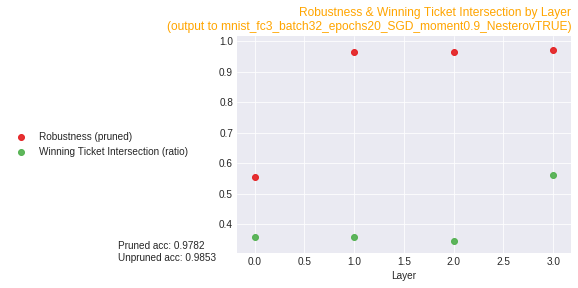
\includegraphics[width=\linewidth]{images/mnist_fc3_robustness_winnery_correlation.png}
  \label{fig:winnery_robustness_correlation}
  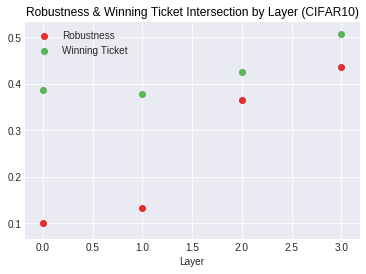
\includegraphics[width=\linewidth]{images/cifar10_fc3_robustness_winnery_correlation.png}
    \caption{Robustness of the pruned layers alongside the size of the intersection with the winning ticket (ratio). Robustness of the unpruned model is almost identical to the pruned robustness (displayed). MNIST accuracy drops from $0.9853$ to $0.9782$ after pruning, and CIFAR10 accuracy drops from $0.4911$ to $0.4794$.}
\end{figure}
While these result seem to show there is no relation between the two phenomenons, examining the robustness patterns on a baseline model (figure \ref{fig:baseline_fc3_heatmap}) and a winning ticket (figure \ref{fig:winnery_robustness}) seem to show an interesting behaviour: Re-initializing the bottom layer on the baseline model drops test accuracy by a 51\%, where on the winning ticket (after pruning) there is a much smaller drop in performance: 25.6\% only. To validate this isn't simply a result of re-initializing a smaller number of weights after pruning, we also pruned the same amount of weights, this time drawn uniformly at random (figure \ref{fig:winnery_robustness}). Random pruning results in a similar robustness pattern as the baseline model (drop in 46\%).\\
This might be since a winning ticket contains a set of well-initialized weights, so that re-initializing weights hurt performance much less than the baseline, and a randomly pruned network.
\begin{figure}
  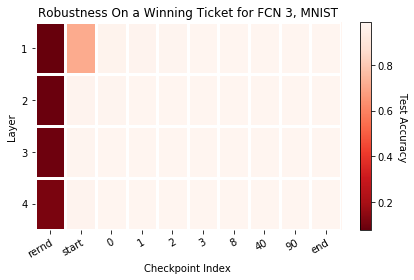
\includegraphics[width=\linewidth]{images/winning_ticket_robustness.png}
  \label{fig:winnery_robustness}
  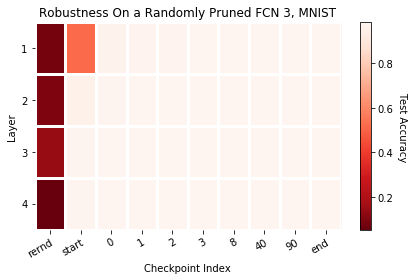
\includegraphics[width=\linewidth]{images/random_pruned_fc3.png}
    \caption{Robustness pattern on a winning ticket and on a randomly pruned network, on a 3-layered fully connected network with MNIST. Baseline robustness pattern appears on figure \ref{fig:baseline_fc3_heatmap}.}
\end{figure}

\section{Applying robustness effect in transfer learning} \label{transfer}

\section{Conclusions and future directions} \label{conclusion}
\bibliography{main}
\bibliographystyle{icml2019}
\end{document}